\section{简谐运动与正弦波} \label{sec:curve-wave}

简谐运动作为最基本的振动模型,
在弹幕中常用来构造振动, 波浪等意象.
简谐运动是一种直线运动,
点在一个固定位置(称为平衡位置)附近做往复运动,
它的位置与时间的关系遵从正弦/余弦函数的规律.
设平衡位置为原点, 简谐运动的表达式为
\[
  x(t) = A\cos(\omega t+\phi),
\]
其图象如图\ref{fig:graph-sine}所示.
该曲线被称为\emph{正弦波}.

\begin{figure}[htbp]
  \centering
  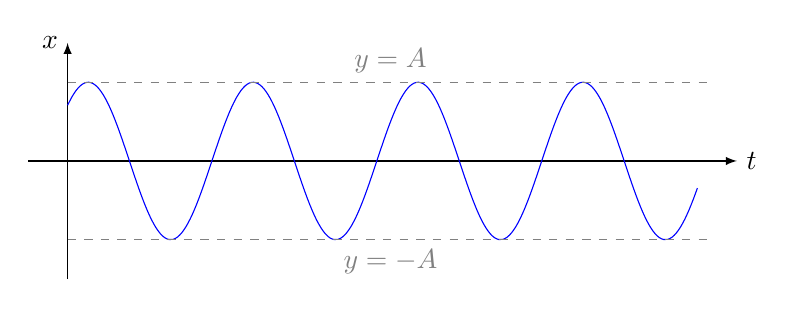
\begin{tikzpicture}
    \draw[-latex] (-0.5,0) -- (8.5,0) node[right] {$t$};
    \draw[-latex] (0,-1.5) -- (0,1.5) node[left] {$x$};
    \draw[smooth,blue,domain={0:8},samples=150]
    plot (\x,{cos((3*\x-pi/4) r)});
    \draw[help lines,dashed] (0,1) -- (8.2,1)
    node[midway,above] {$y=A$};
    \draw[help lines,dashed] (0,-1) -- (8.2,-1)
    node[midway,below] {$y=-A$};
  \end{tikzpicture}
  \caption{简谐运动的图象}
  \label{fig:graph-sine}
\end{figure}

简谐运动可以看作匀速圆周运动在直线上的投影.
设一个点作匀速圆周运动, 圆心为原点, 半径大小为$A$,
初始的角位置为$\phi$, 角速度为$\omega$, 则
\begin{align*}
  \vec r(t) & = \braket{A, \omega t + \phi} \\
  x(t)      & = A\cos(\omega t + \phi)
\end{align*}

也就是说此时点的横坐标进行的就是简谐运动.
在研究简谐运动时, 我们常常借助对应的匀速圆周运动.

在简谐运动$x(t) = A\cos(\omega t + \phi)$中,
$A$等于点与平衡位置的最大距离, 称为简谐运动的\emph{振幅};
$\omega$对应圆周运动的角速度, 在简谐运动中又称为\emph{角频率},
因为$\omega$与运动的频率呈正比例;
$\omega t+\phi$对应圆周运动的角位置,
在简谐运动中称为\emph{相位}, $\phi$称为\emph{初相位}.

简谐运动的速度和加速度等于对应圆周运动的速度和加速度向量的横坐标, 即
\begin{align*}
  v(t) & = A\omega\cos(\omega t+\phi + 90\degree)
  = -A\omega\sin(\omega t+\phi)                   \\
  a(t) & = -A\omega^2\cos(\omega t+\phi)
  = -\omega^2 x(t).
\end{align*}

简谐运动的内容就是这些了, 接下来我们聊点进阶的东西.

\subsubsection{振幅变化的正弦波}

标准的简谐运动/正弦波的振幅是恒定的,
我们可以把振幅$A$替换为函数$A(t)$来构造新的曲线.

缓动函数 (easing functions) 是一类经过点$(0,0),(1,1)$的函数,
用来描述变量从一个值变化到另一个值的变化模式.
\url{https://easings.net/#}展示了一些常见的缓动函数,
其中名为\raw{easeOutElastic}的函数图象如左图所示:

\begin{center}
  \begin{tikzpicture}[scale=2]
    \draw[-latex] (0,0) -- (1.5,0) node[right] {$x$};
    \draw[-latex] (0,0) -- (0,1.5) node[left] {$y$};
    \draw[smooth,blue,domain={0:1},samples=50]
    plot (\x,{1-2^(-10*\x)*cos(\x*10*120)});
    \draw (1pt,1) -- (-1pt,1) node[left] {1};
    \draw (1,1pt) -- (1,-1pt) node[below] {1};
  \end{tikzpicture}
  \begin{tikzpicture}[scale=2]
    \draw[-latex] (0,0) -- (1.5,0) node[right] {$x$};
    \draw[-latex] (0,0) -- (0,1.5) node[left] {$A(x)$};
    \draw[smooth,red,domain={0:1},samples=50]
    plot (\x,{2^(-10*\x)});
    \draw (1pt,1) -- (-1pt,1) node[left] {1};
    \draw (1,1pt) -- (1,-1pt) node[below] {1};
  \end{tikzpicture}
\end{center}

这实际上就是一个振幅变化的正弦波, 对应的函数表达式为
\[
  y = 1 - A(x) \cos(x\cdot1200\degree),
\]
其中振幅函数$A(x) = 2^{-10x}$在$x=0$处的值为1,
在$x=1$处的值约为0, 图象如右图所示.

\subsubsection{李萨如图形}

匀速圆周运动的横坐标做简谐运动,
实际上其纵坐标也做简谐运动, 横纵坐标的简谐运动角速度相等,
只是初相位相差90\degree.
横纵坐标都做简谐运动(角速度和初相位可能不同)的平面运动,
其轨迹曲线称为李萨如图形.

根据横纵坐标角速度以及初相位的不同,
李萨如图形有各种不同的形状, 比如下图的几个例子:

\begin{center}
  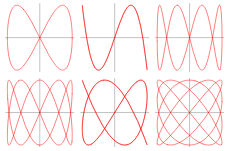
\includegraphics[width=0.5\textwidth]
  {assets/curve/lissajous.png}
\end{center}

不过似乎李萨如图形不太会出现在弹幕中,
这里就不展开细说了.
